\documentclass[english,a4paper]{article}
\usepackage{lmodern}
\usepackage{float}
\usepackage{amssymb,amsmath}
\usepackage{ifxetex,ifluatex}
\usepackage{fixltx2e} % provides \textsubscript
\usepackage[T1]{fontenc}
\usepackage[utf8]{inputenc}
% use upquote if available, for straight quotes in verbatim environments
\IfFileExists{upquote.sty}{\usepackage{upquote}}{}

\usepackage{microtype}
\usepackage[unicode=true]{hyperref}
\usepackage[usenames,dvipsnames]{color}
\hypersetup{breaklinks=true,
            bookmarks=true,
            pdfauthor={},
            pdftitle={},
            colorlinks=true,
            citecolor=blue,
            urlcolor=blue,
            %linkcolor=magenta,
            pdfborder={0 0 0}}
\urlstyle{same}  % don't use monospace font for urls
\usepackage{color}
\usepackage{listings}

\usepackage{longtable,booktabs}
\usepackage{graphicx,grffile}
\makeatletter
\def\maxwidth{\ifdim\Gin@nat@width>\linewidth\linewidth\else\Gin@nat@width\fi}
\def\maxheight{\ifdim\Gin@nat@height>\textheight\textheight\else\Gin@nat@height\fi}
\makeatother
% Scale images if necessary, so that they will not overflow the page
% margins by default, and it is still possible to overwrite the defaults
% using explicit options in \includegraphics[width, height, ...]{}
\setkeys{Gin}{width=\maxwidth,height=\maxheight,keepaspectratio}
\setlength{\parindent}{0pt}
\setlength{\parskip}{6pt plus 2pt minus 1pt}
\setlength{\emergencystretch}{3em}  % prevent overfull lines


% Redefines (sub)paragraphs to behave more like sections
\ifx\subsubsection\undefined\else
\let\oldparagraph\subsubsection
\renewcommand{\subsubsection}[1]{\oldparagraph{#1}\mbox{}}
\fi
\ifx\subparagraph\undefined\else
\let\oldsubparagraph\subparagraph
\renewcommand{\subparagraph}[1]{\oldsubparagraph{#1}\mbox{}}
\fi

\setcounter{secnumdepth}{3}
\setcounter{tocdepth}{3}

\title{Beaker: A security protocol and framework for smart
contracts}\label{beaker-a-security-protocol-and-framework-for-smart-contracts}

\author{Jacob Payne \and Jake O'Shannessy \and Alexey Troitskiy}

\begin{document}

\maketitle

\begin{abstract}\label{abstract}

We describe a secure and extensible operating system for smart
contracts. Using a capability-based exokernel protocol, we can
facilitate secure and low friction peer-to-peer state management across
multiple smart contracts on the Ethereum blockchain. The protocol is
intended to serve as an open standard and building block, establishing
interoperability between contracts that provide 3rd party services and
protocols.

\end{abstract}

\newpage
\tableofcontents
\newpage

\section{Introduction}\label{introduction}
\begin{quote}
``Every program and every privileged user of the system should operate
using the least amount of privilege necessary to complete the job.''

--- Jerome Saltzer, Communications of the ACM
\end{quote}

The underlying idea of decentralized organizations is the use of
blockchain technology to securely manage and track a broad range of
predominantly financial interactions without requiring a trusted third
party.

While lucrative, the development and deployment of such organizations
has a high barrier of entry. Smart contract development practices and
tooling are still in their prenatal stages of maturity, with zero margin
for error. Additionally, organizations must be extensible upfront to
allow changes and upgrades to such protocols and still maintain high
standards of safety.

Beaker is a minimal open-source exokernel protocol that serves as a
building block for establishing secure and scalable organizations.
Beaker enables organizations that will grow in complexity and will
require long term extensibility.

Using Beaker, users can establish an organization on the blockchain with
a much higher level of confidence in it's stability and security. The
safety model Beaker provides not only reduces risk, but allows
organizations to be designed in a much more flexible and robust manner.

The exokernel model of Beaker allows organizations to freely define
their own systems and procedures, but within a safe and controlled
environment. The Beaker kernel provides the building blocks and
primitives that organizations need to build more nuanced governance
models to suit their use case. Most critically, by using the primitives
Beaker provides, designers of these systems will then be able to
demonstrate these security guarantees to others without requiring
manual-code verification.

\section{Problems}\label{problems}
Smart contracts are, by their nature, unforgiving machines that follow
the their specification to the letter. This is one of the selling points
of smart contracts, but it can also be their downfall as the machine
will faithfully execute any flaw or mistake in that code. This is a well
known property of smart contracts, and is tackled in a variety of ways.
By employing lower level primitives like multi-signature wallets or
escrow, the users of smart contracts can build a more flexible and
forgiving system on top of the raw and unforgiving Ethereum machine
underneath.

Building higher level systems however, increases the complexity of the
system one is using. With this complexity comes the risk that one small
error or vulnerability can bring down a whole system. This forces users
to strike a balance between flexibility and complexity.

Another issue, is the lack of transparency within the verification
process itself. While a developer can verify their system themselves,
everyone else using that system simply has to trust that developer. The
users will unlikely have access to the source code, expertise, or even
resources to undertake a sufficient verification of that code, and to
look at the contract on the blockchain is to simply look at a black box.

\section{Existing Work}\label{existing-work}
The design and development of decentralized organizations implemented on
Ethereum have so far failed to be standardized. Due to the generally
highly specialized nature of these systems, most existing service
platforms and protocols developed are highly fragmented, with the design
of the protocol closely linked to the model of the organization it was
designed for.

The lack of a standard model for organizations has so far lead to many
security vulnerabilities. One of the prominent examples was ``The DAO''
that was built to act as a hedge fund with a built-in proposal protocol
to manage funds. The implementation was written in a highly specialized
manner and did not separate the security mechanisms from the business
logic. This lead to a large attack space and ultimately a re-entrancy
vulnerability that allowed the attacker to steal funds from the
organization itself.

Of the recent projects that are making an impact in this area is the
ZeppelinOS ZEP protocol by the Zeppelin Team. Users of smart contract
libraries that use the ZEP protocol are able to vouch or vote for
upgrades they wish to adopt. Only code that is sufficiently vouched for
by the users is included in the system, with the developers working on
that code being rewarded in cryptocurrency assets. The vouching system
ensures that only code that has been approved by all the relevant users
is included and allocates monetary rewards to incentivize high quality
development work.

Unfortunately, this solution only solves a governance problem, which
does not address the issue of limited introspection and transparency of
the contracts themselves. In order to participate in this governance
model, one would need to be able to understand and guarantee that every
byte of code that one approves is correct. While the governance model
gives one power over what code is included and what isn't, it doesn't
equip one with the necessary tools or resources to make good decisions
long-term.

Only highly skilled developers who are familiar with both blockchain
contracts and the system involved have any hope of being able to
understand the detail of code changes, and even they are limited in the
resources they are able to spend on this activity. Regardless of what
promises you are being told, unless you are a developer - the system is
a black box. It requires sophisticated tools to be inspected and
understood; without sufficient resources you cannot verify on your own
how the system is actually implemented. Relying on developers alone - to
verify these systems as we do today - will not be enough to legitimize
smart contracts as secure financial instruments that the mainstream
market can trust long-term.

To solve this, we propose a more general approach by creating an
explicit security model for developing smart contracts that allows
developers the ability to establish semantic restrictions that can
communicate their intentions to their users. As an abstraction,
restrictions that can be easily understood establish transparency and
allow users an ability to verify these contracts on their own without
relying on 3rd party trust.

\section{Overview}\label{overview}
\begin{figure}[H]
    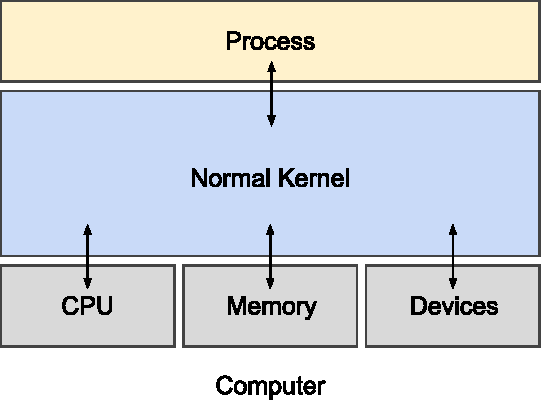
\includegraphics[width=0.49\textwidth]{media/NormalKernelOverview.pdf}
    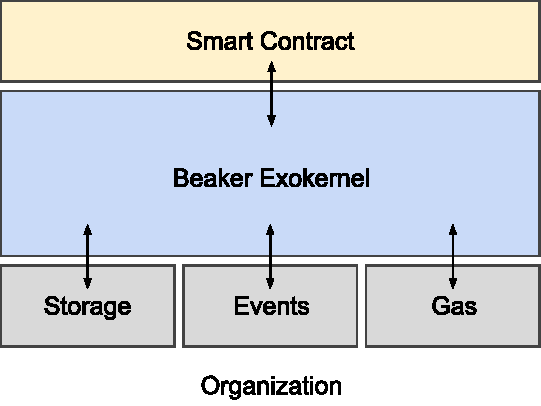
\includegraphics[width=0.49\textwidth]{media/BeakerKernelOverview.pdf}

    \caption{Similar to how existing operating systems act as an
    interface to hardware for applications on a computer, the Beaker kernel
    provides an interface for smart contracts to securely access privileged
    assets and data of an organization.\label{fig:kernels}}
\end{figure}

In their early days, computers executed a sequence of instructions and
manipulated input and output devices, blindly following the instructions
laid out by the programmer. It was up to the programmer to ensure that
the program they wrote was correct. Once the computer was executing the
programmer had relinquished control and the program would execute as
written.

Driven by a need to manage multiple programs, and eventually include
restrictions, quotas and permissions, operating systems were created.
With operating systems, the programs weren't just executed blindly by
the machine. When the machine encountered an instruction that required
hardware access, it suspended the running program and passed that
instruction to the operating system, which then decided what to do. This
gave the operator of the machine control over what was and wasn't
allowed to occur on the machine, at the cost of some run-time
monitoring.

On Ethereum the situation is very similar to those early days of
computers. Smart contracts are thoroughly audited and tested, but once
they are on the blockchain they execute on the raw machine. If we want a
system where we can interpose ourselves between our components and
potentially dangerous resources (such as our storage) we need to make
stronger guarantees about the safety of our system without having to
apply the same level of verification to every component.

In order to do so, we need to require that all contracts interact with
critical resources only through system calls. Once a contract is only
operating through system calls, the operating system kernel has the
final say on what the contract can or cannot do.

\subsection{Procedures}\label{procedures}
A Procedure is a smart contract that can be executed by the kernel.
Unlike normal smart contracts, procedures have several restrictions.
Critically, procedures are only able to access state changes via system
calls, and are not able to directly access storage, make outside calls
or send transactions.

Much like processes are stored in a process table within a traditional
operating system, procedures are stored within a Procedure Table. Each
entry contains the id, capability list and address of the procedure.
Unlike a process table however, the procedure table does not maintain
procedure state across separate transaction calls.

\subsection{On-Chain Code
Verification}\label{on-chain-code-verification}
In order to verify that a procedure follows certain restrictions we use
On-Chain Code Verification, or OCCV for short. OCCV is the use of a
trusted smart contract to read and verify the code of an untrusted smart
contract. By reading an untrusted contract before creation (CREATE
opcode) or after creation (EXTCODECOPY opcode), we can now make
assertions what it can and cannot do.

With OCCV we can check if an untrusted contract has any opcodes that we
don't allow. While this can be limited, this allows us to check if a
contract can potentially: self destruct, make state changes, emit events
or make an external call. This might not seem much, but the absence of
such code allows us to make certain guarantees. For example: if the code
does not contain the combination of SELFDESTRUCT, DELEGATECALL or
CALLCODE, we now know that this code will never be able to be destroyed.

In our case, the trusted contract will be our kernel, while the
untrusted contract would be a procedure. Before running a procedure, the
kernel can check and verify the procedure, allowing the kernel to
enforce certain restrictions or access control. The kernel only needs to
do this check only once however, since in Ethereum the code of a
contract can never change.

\subsection{System Calls}\label{system-calls}
As we covered above, a traditional operating system achieves
introspection and control by interposing itself between the processes
that are running and all other parts of the system including storage,
memory, and even other processes. Each process is given its own memory
and access to a processor, but is otherwise completely isolated. In
order to do even the most fundamental task (be it print a character to
the screen or read some stored data) it must ask the operating system to
do so on its behalf. It is only through the operating system that the
process can affect the real world. Via this mechanism, the kernel has
complete control over what that process can and cannot do. These
requests to the operating system that a process makes are called System
Calls.

The sequence of EVM opcodes below define a Beaker system call. The input
and output parameters of the system call are set prior to these
instructions, and are the responsibility of the designer of the contract
(presumably with significant assistance from libraries).




\definecolor{mygreen}{rgb}{0,0.6,0}
\begin{minipage}{\linewidth}
\begin{lstlisting}[language=c,commentstyle=\color{mygreen},basicstyle=\ttfamily,identifierstyle=\color{blue},caption=Sequence of steps to perform a system call.]
CALLER         // Get Caller
GAS            // Put all the available gas on the stack
DELEGATECALL   // Delegate Call to Caller
\end{lstlisting}
\end{minipage}

These instructions ensure that the contract is only calling to the
original kernel instance and nothing more. Because this sequence of
instructions is the only sequence of instructions with a state changing
opcode (DELEGATECALL) we can use on-chain code verification to prove
that a contract contains no state changing opcodes other than in the
form of a secure system call.

The delegate call is a call back into the kernel. The kernel will only
accept system calls from procedures in its procedure table that it is
currently calling. When a procedure is initially called, it is called
via CALLCODE. This means that that our system, which we will call our
``kernel instance'', is the current storage and event space of the
running code. It also means that the CALLER value, which is a global
read-only value, is set to the address of our kernel instance. When our
procedure does a DELEGATECALL, this address is maintained. As a
consequence, whenever a kernel is executing a system call, it is able to
simply check that the CALLER value is equal to its own address (it is
necessary for this value to be hardcoded into the instance, which is
performed during instantiation).


\begin{figure}[htbp]
\centering
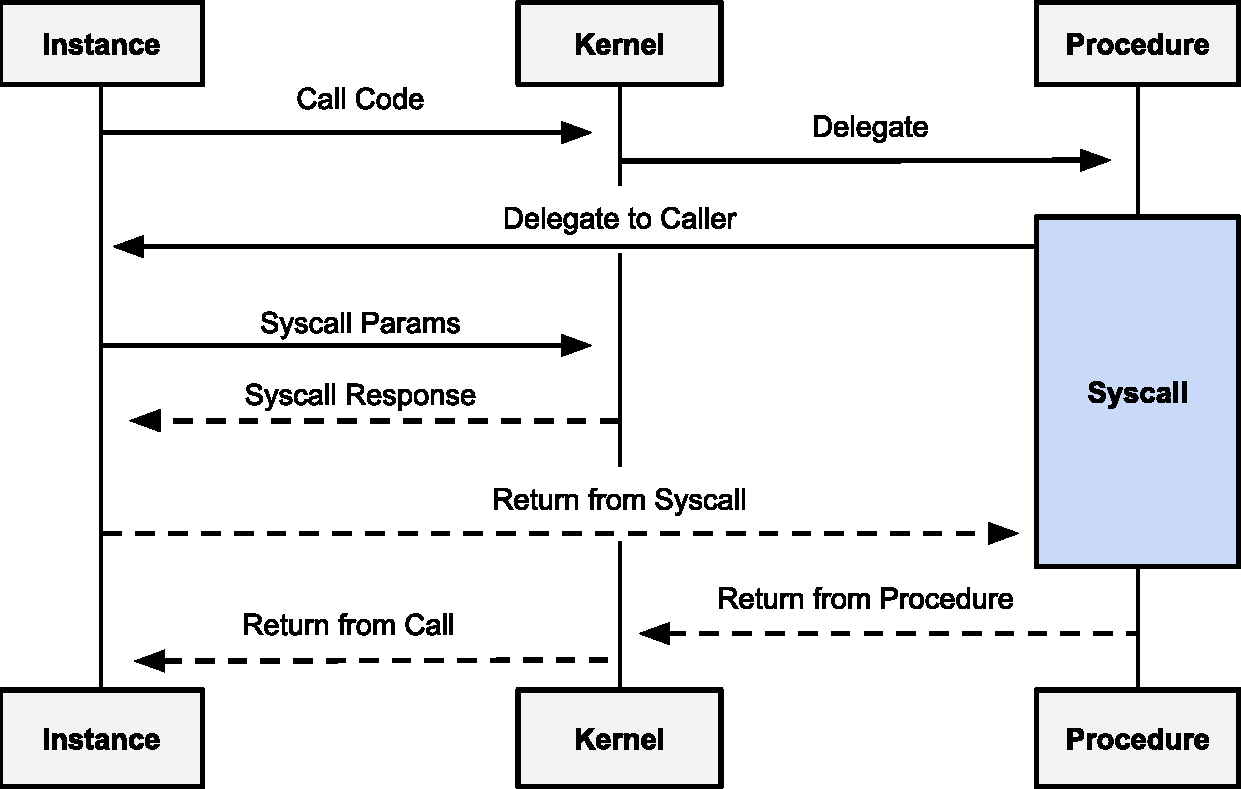
\includegraphics[width=0.8\textwidth]{media/SystemCalls.pdf}
\caption{This diagram illustrates the general sequence of steps
done when a procedure executes a system call}
\end{figure}

\begin{enumerate}
\def\labelenumi{\arabic{enumi}.}
\item
  Kernel instance does a CALLCODE (i.e.~a regular library) to the kernel
  library, executing the function in the kernel library that executes
  procedure.
\item
  The kernel library code uses the procedure table of the kernel
  instance to call the correct procedure using DELEGATECALL. During its
  execution, the procedure encounters a system call and performs a
  DELEGATECALL to the CALLER value, which is the kernel instance.
\item
  The kernel instance checks that itself is the original caller and if
  so, calls the kernel library for processing the system call.
\item
  After the system call is completed, the kernel library returns to the
  kernel instance, which then returns to the procedure.
\end{enumerate}

With this we have a kernel that is generally only accessible from its
own procedures. It must, however, also accept some form of external
transaction, this is the only way it can be triggered to execute code.
As an operating system Beaker should have no say over what kind of
transactions and programs a system wants to execute. Beaker follows a
exokernel design, where the kernel itself should stay out of the user's
code as much as possible.

\subsection{Procedure Creation}\label{procedure-creation}
Creating and adding a procedure to the kernel's procedure table (so that it can
be executed) involves two steps. The first is to create and deploy the procedure
as you would any other smart contract. Once it is deployed, it can then be
registered with the kernel by simply giving the kernel the address of the code
and letting the kernel handle the registration process. During this process, the
kernel will first run the code through the verification process to ensure that
the only state changing code it contains is run through the kernel. If the code
passes this verification process, it is then added to the kernel's procedure
table.

An important feature of this verification process is that it runs on-chain.
Although more expensive then verifying things off-chain, this verification
process is the core mechanism by which the kernel prevents execution of
untrusted opcodes. This verification means that the 'proof' now lies on-chain,
and we aren't simply trusting developers to have done the correct verifications.

\begin{figure}[htbp]
\centering
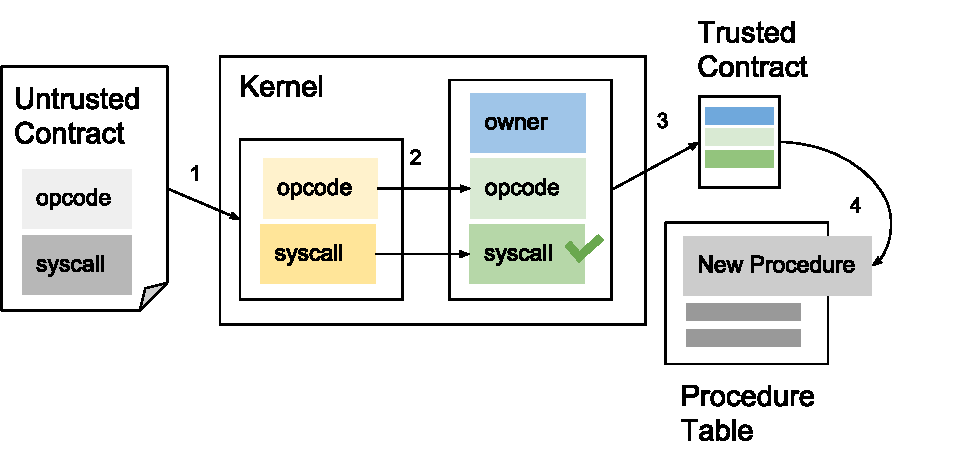
\includegraphics[width=1\textwidth]{media/ProcedureCreation.pdf}
\caption{This diagram illustrates the general sequence of steps to
verify and add protection to the procedure template for it to be
included in the procedure table.}
\end{figure}


\begin{enumerate}
\def\labelenumi{\arabic{enumi}.}
\item
  First, the contract is built and deployed as usual.
\item
  Second, the address of the contract is passed to the kernel for registration.
  The kernel parses the code of this contract and verifies it does not contain
  any illegal opcodes. If any illegal opcodes are found, the contract is
  rejected.
\item
  To designate a syscall dispatch, the code must include a valid syscall
  entry. To allow the kernel ownership, it checks if the contract has an
  additional header that prevents unauthorized calls to the contract.
\item
  Once the code as been verified it is added to the kernel's procedure table,
  and can then be assigned capabilities.
\item
  The procedure can then be used.
\end{enumerate}

\subsection{Entry Procedure}\label{entry-procedure}
We have established that a Beaker kernel instance has to accept two
types of transactions:

\begin{enumerate}
\def\labelenumi{\arabic{enumi}.}
\item
  A System Call, which will come from an executing procedure that the
  kernel itself called earlier.
\item
  An External Call from a 3rd party Ethereum address. This is what will
  trigger whatever actions the designer of the system has chosen to
  implement.
\end{enumerate}

We have covered above how system calls are secured by ensuring that the
kernel only accepts system calls from procedures it is currently
calling. To handle external calls however, we must also establish a way
to handle external transactions.

In order to define an external interface to the kernel, we have a
procedure which is designated as the Entry Procedure. This entry
procedure is created (and updated if need be) by the user, and is
executed as a normal procedure. When the kernel instance receives an
external transaction from another Ethereum address, it simply forwards
the message data to the entry procedure. Thus whenever any transaction
reaches the kernel, it is up to our entry procedure to decide what
should happen and act as the interface to the kernel.

\begin{figure}[htbp]
\centering
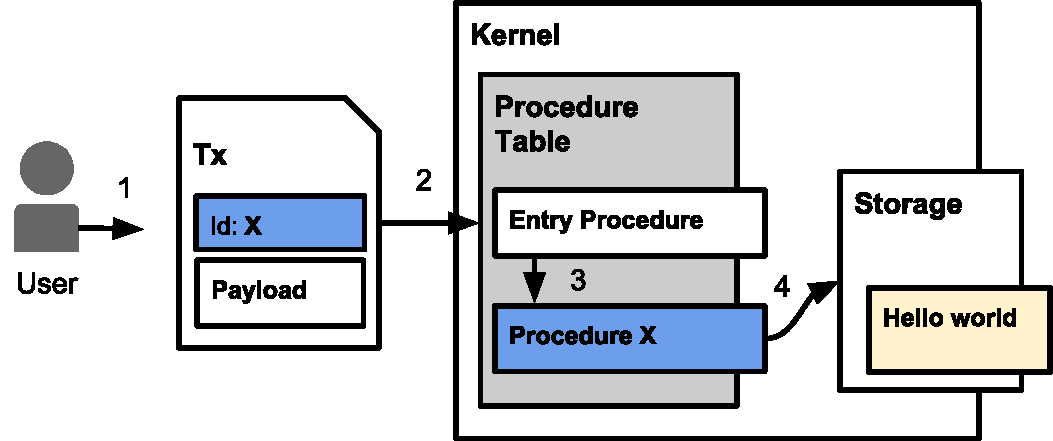
\includegraphics[width=1\textwidth]{media/EntryProcedure.pdf}
\caption{This diagram presents the general sequence of steps used
for executing an entry procedure.}
\end{figure}


\begin{enumerate}
\def\labelenumi{\arabic{enumi}.}
\item
  A user creates an order to execute a procedure. The format is defined
  by the entry procedure, but would usually contain the procedure id,
  and whatever payload the procedure needs.
\item
  The Kernel looks up the entry procedure in the procedure table, and
  dispatches it.
\item
  The entry procedure reads the payload And performs whatever user
  authentication logic the developer of the system desires.
\item
  If the payload is valid, the entry procedure looks up procedure X and
  calls it, procedure X does its primary function, which in this example
  is to store the string ``Hello World'' in storage. This is done using
  a syscall invoked using the necessary capability.
\end{enumerate}

\subsection{Auditability and the Principle of Least
Privilege}\label{auditability-and-the-principle-of-least-privilege}
Existing systems such as DSLs (Domain-Specific Languages) or libraries
offer some level of verification and guarantees. Before the smart
contracts are deployed, the developer is able to use these tools to
verify the contracts. However, once these contracts are deployed they
contain no information that can be used to readily verify the system.
They have become opaque, and the verification information is only
available to the developer.

By using an operating system model, Beaker is able to enforce isolation
at runtime. The information on the isolation of the system is contained
within the kernel and can be audited quite simply be anyone looking at
the system. This allows us to no only isolate the highest risk portion
of our code and reduce our attack surface, but also to verifiably
demonstrate that to others. To an outside auditor, many chunks of a
Beaker system will also be opaque black boxes. The difference is, this
auditor will be able to see which permissions are applied to which black
box. In other words the system becomes a collection of isolated and
restricted black boxes.

Just as when running Linux or any other regular system, it is of course
possible to run all code with full permissions (i.e.~root). All of the
system code can be included in a single procedure with full capabilities
and the system will become as secure as a regular smart contract. But by
applying isolation, Beaker allows developers to separate their system
into specialised components. These components that can then implement
large amounts of logic without the risk of accidentally (or maliciously)
executing some of the more dangerous functions of the system.

In order to do this, we need a security model to apply to procedures and
system calls.

\section{Security Model}\label{security-model}
We established two critical components of the Beaker exokernel:
introspection via system calls, and isolation via procedures to achieve
the principle of least privilege.

System calls establish a way in which the operating system can now allow
or deny various system calls. For this to be used effectively there
needs to be a system for specifying policies. It is these policies that
determine when the kernel should allow or deny a particular action.

In regular computing these restrictions do not generally exist within
programs. It is not possible in most programming languages to import a
library or module and say ``my program sends packets over the network,
and must have permission to do so, but this section of code coming from
this library should not be able to''. This is the state of Ethereum
security currently. Everything is built as a single program, without
internal security boundaries available. (the new STATICCALL opcode is an
attempt to implement this).

However, now that we have established an operating system with system
calls, we now have that point of control over the contracts running on
our system, and we can craft policies to allow or deny any action that
interacts with the rest of the system.

To implement these policies, Beaker uses a capability-based
access-control model. Access control governs all procedures; in order to
perform a system call a procedure must possess an unforgeable token or
key called a Capability. This capability identifies the particular
resource a procedure wants to access, and simply by being in the
procedures possession gives the procedure authority to use that
resource.

\subsection{Criteria for a Policy
Mechanism}\label{criteria-for-a-policy-mechanism}
The tradeoffs in designing a policy mechanism are many. If the policy
mechanism is too simple, it will not be able to provide the necessary
security guarantees. If it is too complex, then the system becomes far
less auditable and almost as complex as the procedures themselves.

Therefore, a policy mechanism must have two critical criteria:

\begin{enumerate}
\def\labelenumi{\arabic{enumi}.}
\item
  It must be simple to read and analyze separately from the code it
  applies to.
\item
  It must be able to represent the guarantees about a system (i.e.~the
  restrictions) that users wish to make.
\end{enumerate}

These two factors are informed by the design already:

\begin{enumerate}
\def\labelenumi{\arabic{enumi}.}
\item
  Given the high stakes and low quantity of code in smart contracts,
  this allows more complex policy mechanisms to be practical, as any
  system deployed as smart contracts must already be heavily audited.
\item
  Beaker follows a microkernel approach so as to give as much freedom to
  the designer as possible. For this reason it is necessary to make as
  few assumptions about the use case of users as possible.
\end{enumerate}

Amongst complex smart contract systems the exact requirements differ
significantly, but the base requirements stay the same. The key goal is
to improve the security and auditability of the system such that an
external party or higher level ``system designer'' might require control
over what the various contracts in the system can do. This would allow
them to compartmentalise areas of code and ensure that it only has the
privileges it requires, allowing them to focus attention on more
critical high-risk code. Even if another member of the organization
updates a contract under his or her control, the system designer should
be able to limit the potential damage of an error or malign action by
sandboxing that contract.

The goal of the security model then becomes to design a system that can
make these guarantees, and present it to those designing or auditing the
system in such a way that they can be checked using fewer resources and
less knowledge.

As an example: in the Linux kernel, the permission bit mask and owner on
a user's personal file allows them to quickly and easily see (by listing
the properties of their files with \texttt{ls\ -l}) that only they, and
anybody with root access can access their files. The simple string
presented by \texttt{ls\ -l} of
\texttt{-rw-r-\/-\/-\/-\/-\ bob\ users\ file.txt} instantly tells
\texttt{bob} that (with the exception of root) only he can modify
\texttt{file.txt}, while other users in the group users can also read
it, but nobody else has access. This short simple string forms the
policy placed on that file. It's simplicity means that the restrictions
placed on that file are easily verifiable. It is not necessary to verify
all the code on the system, because we know that the Linux kernel will
enforce this policy.

\subsection{Implementing a Capability Based Security
Model}\label{implementing-a-capability-based-security-model}
All policies in Beaker are applied directly to procedures. Beaker is a
capability-based OS and therefore the policies take the form of a
Capability List. Each capability in this list is an unforgeable key.
This key is both an identifier for a resource, and an inherent
permission to access that resource. The procedure cannot act outside
this set of capabilities. Even if the procedure is updated, the limits
of the procedure do not expand unless the capabilities associated with
that procedure also expand.

By applying these capabilities at a procedure level, the policy
mechanism becomes very simple. Where more complex policies are required,
they can often be modelled by using simple procedures that ``become''
the policies and can be more simply audited.

It is critical to note that the capability system proposed here does not
attempt to deal at all with ``users''. If a particular system includes
users (which is to be expected) it is left to the creators of that
system to dictate how that is organised and implemented.

For this reason, Beaker aims to help system designers implement their
own higher level permissions systems on solid primitives, rather than to
anticipate all the use cases for those using Beaker.

Presented here is an outline of what a simplistic capability system
might look like in Beaker. A procedure is created in two steps:

\begin{itemize}
\item
  Creation/Update: where the contract bytecode is uploaded to the
  kernel.
\item
  Permission assignation: where somebody with the appropriate capability
  sets the capabilities of the new procedure.
\end{itemize}

When a procedure is created, it has zero capabilities available to it in
its list. If, for example, it needs to modify the storage value at 0x7,
it will need to be provided with that permission by a separate
permission assignation. In this workflow, the procedure is deployed by a
developer, and the permissions are assigned by the system designer once
he approves this. The workflow around how permissions are requested and
designed are left to the users.

The advantage of this design, where capabilities are assigned to
procedures, is that it is simple and enforceable. Compared to some other
capability system designs this does have a few limitations. One
limitation it does not support dynamically chosen capabilities. For
example this means that it is not possible to pass a capability of a
particular storage location to a procedure. This is an often touted
feature of capability systems that allows for the delegation of
authority. The advantage of eschewing such a feature is that it makes
the capabilities more static and auditable.

\subsection{Custom User Permissions}\label{custom-user-permissions}
A capability-based security model allows the flexibility to define a
procedure that can act as a custom permission system akin to an access
control list. With a custom permission system, users are free do define
their own hierarchies or groups in order to satisfy their particular
requirements. Thus users are not forced to follow a specific permission
model that does not fit their needs and still maintain safety through
establishing explicit access control within the system.

\begin{figure}[htbp]
\centering
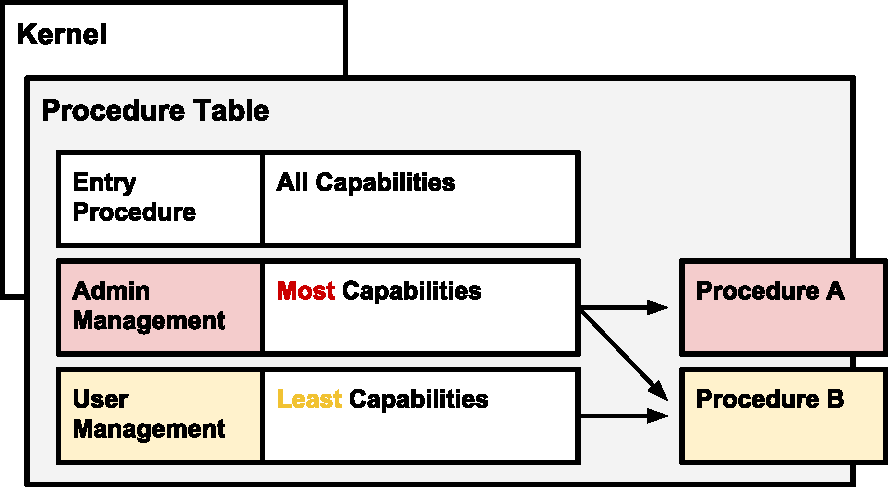
\includegraphics[width=1\textwidth]{media/Separation.pdf}
\caption{By separating admin management from user management, the
principle of least authority can be applied.}
\end{figure}

An example access model can involve group decision making by vote, where
a procedure is created to check votes and dispatch actions on resources
within its allowed capabilities. Such a procedure can act as an
administration system to maintain and upgrade previously defined
components within the organization by secure vote.

Another example can involve groups. Where group is assigned control over
a procedure with designated capabilities that define how the group can
affect the organization. This in effect can be used as an explicit
safeguard where each group cannot compromise the other's resources.

\subsection{Kernel Objects}\label{kernel-objects}
\begin{table}[H]
    \caption{Kernel objects.}
    \centering{}%
    % \begin{tabular}{>{\centering}p{0.25\textwidth}|>{\centering}p{0.475\textwidth}|>{\centering}p{0.2\textwidth}}
    \begin{tabular}{l|l|p{0.5\textwidth}}


        \hline
        Kernel Object & Capability Type & Description\tabularnewline
        \hline
        \hline
        Procedure & create & Create procedure with given
        identifier.\tabularnewline
        & push\_cap & Add capability to procedure with given
        identifier\tabularnewline
        & delete\_cap & Delete capability from procedure with given identifier
        and index\tabularnewline
        & call & Call procedure by given id and arguments.\tabularnewline
        & delete & Delete procedure by identifier.\tabularnewline
        & entry & Set the procedure with given identifier as the entry
        procedure.\tabularnewline
        \hline
        Storage & read & Read from the memory by the given
        address.\tabularnewline
        & write & Write to the memory by the given address.\tabularnewline
        \hline
        Log & write & Append log record with given topics.\tabularnewline
        \hline
        Gas & received & The total amount of gas received from
        user.\tabularnewline
        & send & Send gas to an external address.\tabularnewline
        \hline
    \end{tabular}
\end{table}

Each Kernel Object is a category of related capability types. Kernel
objects designate the resources in the kernel that are protected by the
kernel reference monitor and can only be indirectly accessed by invoking
a system call.

\subsubsection{Procedure Table}\label{procedure-table}
Sometimes, procedures need to access information about themselves as
well as the state of the kernel. This includes the capabilities it has
available as well as finding what other procedures are available. It is
also important for procedures to able to dispatch other procedures if
they are allowed to do so. This is usually when a procedure is used as a
policy to check and verify if the appropriate signatures have been done.
The procedure table object is a dynamic list of procedure identifiers
that designate what procedures the kernel has available. Each procedure
is defined by a unique identifier, contract address and a capability
list.

\subsubsection{Storage}\label{storage}
Storage is the only way procedures can store and modify data. However,
allowing procedures to directly access storage is unsafe and would
inadvertently allow procedures to access or modify data that they do not
own. To prevent this, storage is abstracted into capabilities that
provide a separate key ranges for each procedure that they are allowed
to modify. Additionally, procedures can provide access to other
procedures to share or modify tables that they own.

The Storage object is defined by a 32 byte storage location where a
procedure can either read or write a 32 byte value. In order to provide
the kernel a protected storage space, storage is divided into two
spaces, with half of locations assigned to kernel-space and and the
other half assigned to user-space storage. This provides all procedure a
user-space of $2^{255}$ unique keys. The number of storage keys far outweighs
the capacity of the storage system itself, so will not be a limiting
factor long term.

\subsubsection{Events}\label{events}
Events are crucial for signalling verified changes to the outside world,
accessing data asynchronously, as well as their use in establishing
off-chain networks. In Ethereum, logs can be ascribed from 0-4 topics,
with each topic being a 32-byte value. These topics are handled as
addresses or namespaces. In order to log to specific topic, the
procedure must have the capability to do so. This capability is the
write capability included under the Log object in the table kernel
object table above. This capability type is then refined to dictate
which topics it can write to.

\subsubsection{Gas}\label{gas}
The Gas object is defined as the total gas resources the kernel has
available and designates how much resources are allocated to a procedure
to spend during execution as well as how much gas it is allowed to send
to an external address.

\section{Summary}\label{summary}
The Beaker exokernel protocol provides a secure environment for
organizations to establish extendible business logic through restricted
smart contracts defined as procedures.

By using a low level capability-based security model, Beaker allows
developers to design custom permissions and policies that suit their use
case, rather than lock organizations into a particular governance model.
These will also form a standard set of primitives that can be used to
reduce the burden of verification and communicate the security design of
the system to others in a transparent manner.

\section{Acknowledgments}\label{acknowledgments}
We would like to express our gratitude to other projects notably our
mentors and advisors, and the many welcoming people in the Ethereum
community.

\end{document}
